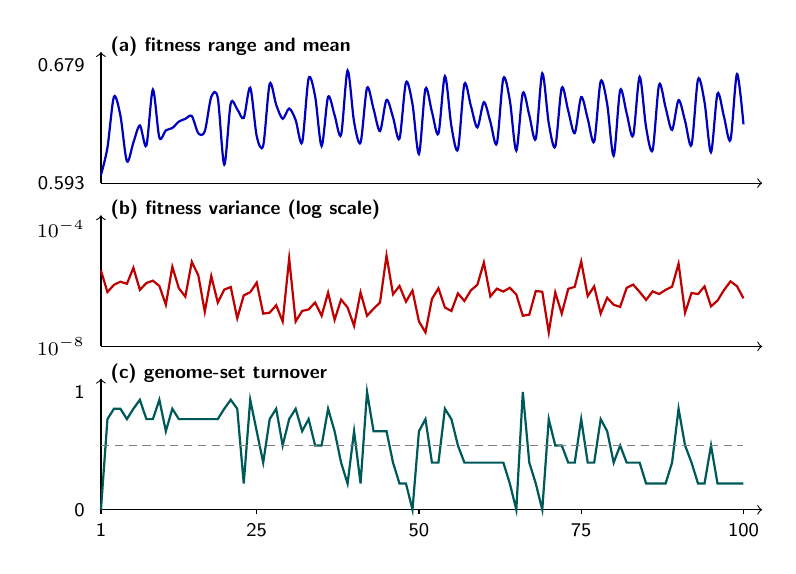
\begin{tikzpicture}[x=0.68cm,y=0.68cm,font=\sffamily\scriptsize]
% Panel A
\begin{scope}[shift={(0,6.1)}]
\draw[->] (0,0) -- (12.35,0);
\draw[->] (0,0) -- (0,2.45);
\fill[blue!12] (0.0000,0.2448) (0.1212,0.7045) (0.2424,1.6724) (0.3636,1.3293) (0.4848,0.4650) (0.6061,0.8637) (0.7273,1.1290) (0.8485,0.7570) (0.9697,1.8093) (1.0909,0.8932) (1.2121,1.0022) (1.3333,1.1373) (1.4545,1.1966) (1.5758,1.2299) (1.6970,1.3833) (1.8182,1.0064) (1.9394,0.9881) (2.0606,1.6754) (2.1818,1.6133) (2.3030,0.3934) (2.4242,1.5508) (2.5455,1.3950) (2.6667,1.2589) (2.7879,1.8183) (2.9091,0.9305) (3.0303,0.7107) (3.1515,1.8732) (3.2727,1.4899) (3.3939,1.2152) (3.5152,1.4814) (3.6364,1.1947) (3.7576,0.7771) (3.8788,1.9755) (4.0000,1.6379) (4.1212,0.7073) (4.2424,1.6491) (4.3636,1.2798) (4.4848,0.9266) (4.6061,2.1185) (4.7273,1.1519) (4.8485,0.7812) (4.9697,1.7895) (5.0909,1.4002) (5.2121,0.9918) (5.3333,1.6483) (5.4545,1.2557) (5.5758,0.8665) (5.6970,1.8909) (5.8182,1.5017) (5.9394,0.5573) (6.0606,1.7694) (6.1818,1.3571) (6.3030,0.9679) (6.4242,2.0196) (6.5455,1.0778) (6.6667,0.6587) (6.7879,1.8670) (6.9091,1.4778) (7.0303,1.0886) (7.1515,1.5673) (7.2727,1.1686) (7.3939,0.7794) (7.5152,1.9876) (7.6364,1.5792) (7.7576,0.6348) (7.8788,1.6925) (8.0000,1.2852) (8.1212,0.8592) (8.2424,2.0754) (8.3636,1.1286) (8.4848,0.7177) (8.6061,1.7957) (8.7273,1.3845) (8.8485,0.9772) (8.9697,1.6624) (9.0909,1.2242) (9.2121,0.8169) (9.3333,1.9199) (9.4545,1.5025) (9.5758,0.5332) (9.6970,1.7495) (9.8182,1.3422) (9.9394,0.9349) (10.0606,2.0090) (10.1818,1.0585) (10.3030,0.6513) (10.4242,1.8675) (10.5455,1.4415) (10.6667,1.0342) (10.7879,1.6002) (10.9091,1.1766) (11.0303,0.7505) (11.1515,1.9668) (11.2727,1.5595) (11.3939,0.6090) (11.5152,1.6859) (11.6364,1.2758) (11.7576,0.8686) (11.8788,2.0848) (12.0000,1.1155) (12.0000,1.0752) (11.8788,1.9812) (11.7576,0.7521) (11.6364,1.2019) (11.5152,1.6510) (11.3939,0.5588) (11.2727,1.4539) (11.1515,1.9020) (11.0303,0.6711) (10.9091,1.1498) (10.7879,1.4312) (10.6667,0.9610) (10.5455,1.3827) (10.4242,1.8128) (10.3030,0.5885) (10.1818,1.0092) (10.0606,1.9537) (9.9394,0.8490) (9.8182,1.2564) (9.6970,1.7038) (9.5758,0.4828) (9.4545,1.4533) (9.3333,1.8886) (9.2121,0.7192) (9.0909,1.1705) (8.9697,1.4690) (8.8485,0.9017) (8.7273,1.2960) (8.6061,1.7611) (8.4848,0.6503) (8.3636,1.1107) (8.2424,2.0187) (8.1212,0.7948) (8.0000,1.2575) (7.8788,1.6709) (7.7576,0.5811) (7.6364,1.5138) (7.5152,1.9235) (7.3939,0.7085) (7.2727,1.1183) (7.1515,1.3833) (7.0303,1.0062) (6.9091,1.4080) (6.7879,1.8173) (6.6667,0.5775) (6.5455,1.0442) (6.4242,1.9795) (6.3030,0.8927) (6.1818,1.2996) (6.0606,1.7533) (5.9394,0.5363) (5.8182,1.4400) (5.6970,1.8492) (5.5758,0.7888) (5.4545,1.1940) (5.3333,1.4458) (5.2121,0.9512) (5.0909,1.3690) (4.9697,1.7660) (4.8485,0.7221) (4.7273,1.1313) (4.6061,2.0852) (4.4848,0.8804) (4.3636,1.2552) (4.2424,1.5823) (4.1212,0.6809) (4.0000,1.5891) (3.8788,1.9375) (3.7576,0.7430) (3.6364,1.1675) (3.5152,1.2762) (3.3939,1.1883) (3.2727,1.4432) (3.1515,1.8407) (3.0303,0.6822) (2.9091,0.8397) (2.7879,1.7399) (2.6667,1.1807) (2.5455,1.3671) (2.4242,1.4522) (2.3030,0.3066) (2.1818,1.5732) (2.0606,1.5424) (1.9394,0.9552) (1.8182,0.8609) (1.6970,1.1448) (1.5758,1.1756) (1.4545,1.1142) (1.3333,0.9144) (1.2121,0.9679) (1.0909,0.8038) (0.9697,1.6912) (0.8485,0.6535) (0.7273,1.0449) (0.6061,0.6595) (0.4848,0.3564) (0.3636,1.2168) (0.2424,1.5719) (0.1212,0.6198) (0.0000,0.0815) -- cycle;
\draw[blue!75!black,thick] plot[smooth] coordinates {(0.0000,0.1524) (0.1212,0.6614) (0.2424,1.6118) (0.3636,1.2593) (0.4848,0.4081) (0.6061,0.7587) (0.7273,1.0771) (0.8485,0.7010) (0.9697,1.7470) (1.0909,0.8504) (1.2121,0.9857) (1.3333,1.0292) (1.4545,1.1483) (1.5758,1.1997) (1.6970,1.2524) (1.8182,0.9318) (1.9394,0.9680) (2.0606,1.6123) (2.1818,1.5940) (2.3030,0.3452) (2.4242,1.4870) (2.5455,1.3783) (2.6667,1.2178) (2.7879,1.7832) (2.9091,0.8785) (3.0303,0.7010) (3.1515,1.8535) (3.2727,1.4639) (3.3939,1.2013) (3.5152,1.3939) (3.6364,1.1779) (3.7576,0.7592) (3.8788,1.9552) (4.0000,1.6196) (4.1212,0.6942) (4.2424,1.6102) (4.3636,1.2702) (4.4848,0.9013) (4.6061,2.1021) (4.7273,1.1458) (4.8485,0.7572) (4.9697,1.7772) (5.0909,1.3851) (5.2121,0.9727) (5.3333,1.5541) (5.4545,1.2317) (5.5758,0.8306) (5.6970,1.8788) (5.8182,1.4762) (5.9394,0.5447) (6.0606,1.7615) (6.1818,1.3302) (6.3030,0.9243) (6.4242,1.9987) (6.5455,1.0607) (6.6667,0.6298) (6.7879,1.8491) (6.9091,1.4417) (7.0303,1.0399) (7.1515,1.5123) (7.2727,1.1451) (7.3939,0.7408) (7.5152,1.9550) (7.6364,1.5470) (7.7576,0.6071) (7.8788,1.6820) (8.0000,1.2681) (8.1212,0.8277) (8.2424,2.0493) (8.3636,1.1174) (8.4848,0.6815) (8.6061,1.7796) (8.7273,1.3492) (8.8485,0.9330) (8.9697,1.6073) (9.0909,1.2026) (9.2121,0.7762) (9.3333,1.9015) (9.4545,1.4771) (9.5758,0.5112) (9.6970,1.7359) (9.8182,1.3045) (9.9394,0.8850) (10.0606,1.9845) (10.1818,1.0383) (10.3030,0.6160) (10.4242,1.8374) (10.5455,1.4118) (10.6667,0.9932) (10.7879,1.5509) (10.9091,1.1609) (11.0303,0.7137) (11.1515,1.9395) (11.2727,1.5119) (11.3939,0.5774) (11.5152,1.6717) (11.6364,1.2383) (11.7576,0.8097) (11.8788,2.0375) (12.0000,1.0971)};
\node[anchor=west,font=\sffamily\bfseries\scriptsize] at (0,2.55) {(a) fitness range and mean};
\node[anchor=east] at (-0.12,0) {0.593};
\node[anchor=east] at (-0.12,2.2) {0.679};
\end{scope}
% Panel B
\begin{scope}[shift={(0,3.05)}]
\draw[->] (0,0) -- (12.35,0);
\draw[->] (0,0) -- (0,2.45);
\draw[red!75!black,thick] plot coordinates {(0.0000,1.4183) (0.1212,1.0148) (0.2424,1.1494) (0.3636,1.2093) (0.4848,1.1699) (0.6061,1.4676) (0.7273,1.0555) (0.8485,1.1838) (0.9697,1.2281) (1.0909,1.1292) (1.2121,0.7782) (1.3333,1.4873) (1.4545,1.0877) (1.5758,0.9296) (1.6970,1.5800) (1.8182,1.3273) (1.9394,0.6469) (2.0606,1.3131) (2.1818,0.8202) (2.3030,1.0612) (2.4242,1.1094) (2.5455,0.5248) (2.6667,0.9528) (2.7879,1.0114) (2.9091,1.1920) (3.0303,0.6127) (3.1515,0.6304) (3.2727,0.7689) (3.3939,0.4648) (3.5152,1.6402) (3.6364,0.4648) (3.7576,0.6623) (3.8788,0.6904) (4.0000,0.8202) (4.1212,0.5728) (4.2424,1.0043) (4.3636,0.4967) (4.4848,0.8751) (4.6061,0.7272) (4.7273,0.3844) (4.8485,1.0079) (4.9697,0.5728) (5.0909,0.7033) (5.2121,0.8202) (5.3333,1.6965) (5.4545,0.9740) (5.5758,1.1292) (5.6970,0.8352) (5.8182,1.0437) (5.9394,0.4648) (6.0606,0.2624) (6.1818,0.8870) (6.3030,1.0852) (6.4242,0.7272) (6.5455,0.6623) (6.6667,0.9896) (6.7879,0.8492) (6.9091,1.0467) (7.0303,1.1514) (7.1515,1.5665) (7.2727,0.9344) (7.3939,1.0775) (7.5152,1.0248) (7.6364,1.0952) (7.7576,0.9699) (7.8788,0.5728) (8.0000,0.5935) (8.1212,1.0344) (8.2424,1.0215) (8.3636,0.2624) (8.4848,1.0079) (8.6061,0.6127) (8.7273,1.0748) (8.8485,1.1139) (8.9697,1.5851) (9.0909,0.9392) (9.2121,1.1206) (9.3333,0.6127) (9.4545,0.9093) (9.5758,0.7782) (9.6970,0.7383) (9.8182,1.0927) (9.9394,1.1552) (10.0606,1.0182) (10.1818,0.8689) (10.3030,1.0281) (10.4242,0.9780) (10.5455,1.0555) (10.6667,1.1162) (10.7879,1.5441) (10.9091,0.6304) (11.0303,0.9971) (11.1515,0.9780) (11.2727,1.1206) (11.3939,0.7490) (11.5152,0.8560) (11.6364,1.0526) (11.7576,1.2152) (11.8788,1.1249) (12.0000,0.8984)};
\node[anchor=west,font=\sffamily\bfseries\scriptsize] at (0,2.55) {(b) fitness variance (log scale)};
\node[anchor=east] at (-0.12,0) {$10^{-8}$};
\node[anchor=east] at (-0.12,2.2) {$10^{-4}$};
\end{scope}
% Panel C
\begin{scope}[shift={(0,0)}]
\draw[->] (0,0) -- (12.35,0);
\draw[->] (0,0) -- (0,2.45);
\draw[teal!70!black,thick] plot coordinates {(0.0000,0.0000) (0.1212,1.6923) (0.2424,1.8857) (0.3636,1.8857) (0.4848,1.6923) (0.6061,1.8857) (0.7273,2.0533) (0.8485,1.6923) (0.9697,1.6923) (1.0909,2.0533) (1.2121,1.4667) (1.3333,1.8857) (1.4545,1.6923) (1.5758,1.6923) (1.6970,1.6923) (1.8182,1.6923) (1.9394,1.6923) (2.0606,1.6923) (2.1818,1.6923) (2.3030,1.8857) (2.4242,2.0533) (2.5455,1.8857) (2.6667,0.4889) (2.7879,2.0533) (2.9091,1.4667) (3.0303,0.8800) (3.1515,1.6923) (3.2727,1.8857) (3.3939,1.2000) (3.5152,1.6923) (3.6364,1.8857) (3.7576,1.4667) (3.8788,1.6923) (4.0000,1.2000) (4.1212,1.2000) (4.2424,1.8857) (4.3636,1.4667) (4.4848,0.8800) (4.6061,0.4889) (4.7273,1.4667) (4.8485,0.4889) (4.9697,2.2000) (5.0909,1.4667) (5.2121,1.4667) (5.3333,1.4667) (5.4545,0.8800) (5.5758,0.4889) (5.6970,0.4889) (5.8182,0.0000) (5.9394,1.4667) (6.0606,1.6923) (6.1818,0.8800) (6.3030,0.8800) (6.4242,1.8857) (6.5455,1.6923) (6.6667,1.2000) (6.7879,0.8800) (6.9091,0.8800) (7.0303,0.8800) (7.1515,0.8800) (7.2727,0.8800) (7.3939,0.8800) (7.5152,0.8800) (7.6364,0.4889) (7.7576,0.0000) (7.8788,2.2000) (8.0000,0.8800) (8.1212,0.4889) (8.2424,0.0000) (8.3636,1.6923) (8.4848,1.2000) (8.6061,1.2000) (8.7273,0.8800) (8.8485,0.8800) (8.9697,1.6923) (9.0909,0.8800) (9.2121,0.8800) (9.3333,1.6923) (9.4545,1.4667) (9.5758,0.8800) (9.6970,1.2000) (9.8182,0.8800) (9.9394,0.8800) (10.0606,0.8800) (10.1818,0.4889) (10.3030,0.4889) (10.4242,0.4889) (10.5455,0.4889) (10.6667,0.8800) (10.7879,1.8857) (10.9091,1.2000) (11.0303,0.8800) (11.1515,0.4889) (11.2727,0.4889) (11.3939,1.2000) (11.5152,0.4889) (11.6364,0.4889) (11.7576,0.4889) (11.8788,0.4889) (12.0000,0.4889)};
\draw[densely dashed,gray] (0,1.2) -- (12,1.2);
\node[anchor=west,font=\sffamily\bfseries\scriptsize] at (0,2.55) {(c) genome-set turnover};
\node[anchor=east] at (-0.12,0) {0};
\node[anchor=east] at (-0.12,2.2) {1};
\foreach \g in {1,25,50,75,100} {\pgfmathsetmacro{\gx}{(\g-1)/99*12} \draw (\gx,0) -- (\gx,-0.08) node[below]{\g};}
\end{scope}
\end{tikzpicture}
